\documentclass{article}

\usepackage{amsmath, amsthm, amssymb, amsfonts}
\usepackage{tikz-cd}
\usepackage{thmtools}
\usepackage{graphicx}
\usepackage{setspace}
\usepackage{geometry}
\usepackage{float}
\usepackage{hyperref}
\usepackage[utf8]{inputenc}
\usepackage[english]{babel}
\usepackage{framed}
\usepackage[dvipsnames]{xcolor}
\usepackage{tcolorbox}
\usepackage{tikz}
\usetikzlibrary{patterns}
\colorlet{LightGray}{White!90!Periwinkle}
\colorlet{LightOrange}{Orange!15}
\colorlet{LightGreen}{Green!15}

\newcommand{\HRule}[1]{\rule{\linewidth}{#1}}

\declaretheoremstyle[name=,]{thmsty}
\declaretheorem[style=thmsty,numberwithin=section]{theorem}
\tcolorboxenvironment{theorem}{colback=LightGray}

\declaretheoremstyle[name=,]{prosty}
\declaretheorem[style=prosty,numberlike=theorem]{notes}
\tcolorboxenvironment{proposition}{colback=LightOrange}

\declaretheoremstyle[name=,]{prcpsty}
\declaretheorem[style=prcpsty,numberlike=theorem]{question}
\tcolorboxenvironment{principle}{colback=LightGreen}

\setstretch{1.2}
\geometry{
    textheight=9in,
    textwidth=5.5in,
    top=1in,
    headheight=12pt,
    headsep=25pt,
    footskip=30pt
}

% ------------------------------------------------------------------------------

\begin{document}

% ------------------------------------------------------------------------------
% Cover Page and ToC
% ------------------------------------------------------------------------------

\title{ \normalsize \textsc{Lie Groups and Lie Algebra}
		\\ [2.0cm]
		\HRule{1.5pt} \\
        \LARGE \textbf{\uppercase{A lecture note on SuperConductivity for Noob Wannabe Physicists}
		\HRule{2.0pt} \\ [0.6cm] \LARGE{} \vspace*{10\baselineskip}}
		}
        %\date{}
\author{\textbf{Author} \\ 
		Mushrafi Munim Sushmit \\
		Department of Physics, University of Dhaka \\
		}

\maketitle
\newpage

\tableofcontents
\newpage

\section*{Preface} % The asterisk prevents LaTeX from numbering the section
\addcontentsline{toc}{section}{Preface} 

This document draws primarily from the online lectures delivered by Dr. Ratan Chandra Ghosh, which are available on YouTube.
\newpage 

\section{Introduction}

In 1911, Heike Kamerlingh Onnes discovered that the electrical resistance of mercury abruptly drops to zero when cooled below a critical temperature of approximately 4.2\,K. This phenomenon, known as \emph{superconductivity}, marked the first observation of perfect electrical conductivity in materials at very low temperatures.

In 1933, Walther Meissner and Robert Ochsenfeld observed that a superconductor expels all magnetic fields from its interior when cooled below its critical temperature, a phenomenon now referred to as the \emph{Meissner effect}. This finding demonstrated that superconductivity is not only characterized by zero electrical resistance but also exhibits unique magnetic properties.

In a superconductor, the magnetic field \(\vec{B}\) is related to the magnetic field intensity \(\vec{H}\) and the magnetization \(\vec{M}\) by the equation:
\[
\vec{B} = \vec{H} + 4\pi \vec{M}
\]
Since \(\vec{B} = 0\) inside a superconductor, the magnetic susceptibility \(\chi\) is given by:
\[
\chi = \frac{\partial M}{\partial H} = -\frac{1}{4\pi}
\]
This shows that a superconductor is a perfect diamagnet.

\begin{figure}
    \begin{center}
        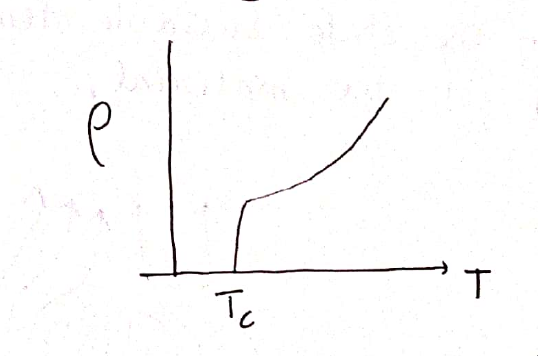
\includegraphics[width=0.5\textwidth]{figures/1.png}
    \end{center}
    \caption{Superconductivity in Mercury}\label{fig:}
\end{figure}


Onnes also found that the superconducting transition is reversible. When he heated the superconducting material, it recovered its normal resistivity at the transition temperature, \(T_c\). This behavior confirmed that the superconducting state is a new state of matter, as it depends on the state variable temperature, not on the history of the material.

\begin{figure}
    \begin{center}
        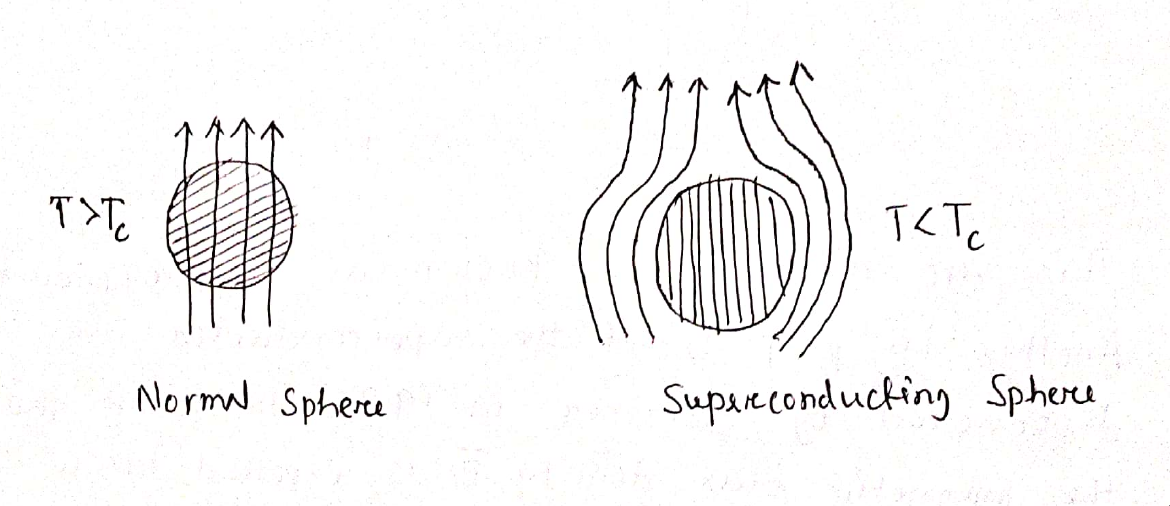
\includegraphics[width=0.95\textwidth]{figures/2.png}
    \end{center}
    \caption{Normal and Superconducting Spheres}\label{fig:}
\end{figure}


\section{Critical Field}

Shortly after his discovery, Onnes also observed that superconductivity can be destroyed by the application of a magnetic field. When a strong enough magnetic field, known as the \emph{critical field}, is applied to a superconducting material, it becomes normal and recovers its normal resistivity, even at temperatures below \(T_c\). This demonstrated that superconductivity is sensitive to external magnetic fields.

\section{Empirical Relation for Critical Field}

The critical magnetic field \(H_c(T)\) depends on the temperature and is given by the empirical relation:
\[
H_c(T) = H_c(0) \left[ 1 - \left( \frac{T}{T_c} \right)^2 \right]
\]
From this equation, it can be observed that the critical field is maximum at \(T = 0 \, \text{K}\) and vanishes at \(T = T_c\).

\begin{figure}
    \begin{center}
        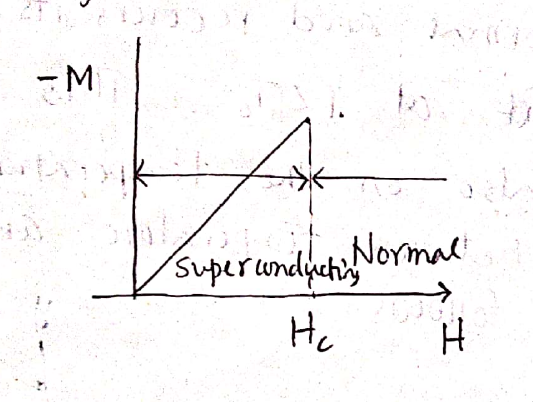
\includegraphics[width=0.95\textwidth]{figures/3.png}
    \end{center}
    \caption{Type-1 Superconductors}\label{fig:}
\end{figure}

\begin{figure}
    \begin{center}
        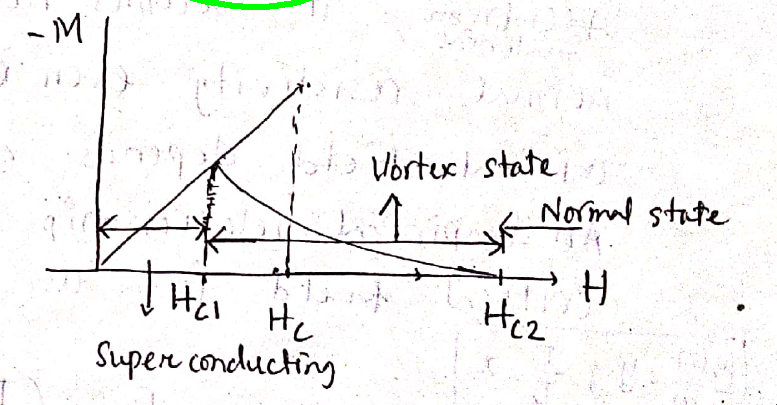
\includegraphics[width=0.95\textwidth]{figures/4.png}
    \end{center}
    \caption{Type-2 Superconductors}\label{fig:}
\end{figure}

\section{Type I and Type II Superconductors}

In \emph{type I} superconductors, there is no intermediate state separating the transition from the superconducting to the normal state upon increasing the magnetic field. The transition occurs directly once the critical field is exceeded.

On the other hand, in \emph{type II} superconductors, there is an intermediate state, called the \emph{mixed state}, which appears before the transition to the normal state. In this mixed state, magnetic flux partially penetrates the superconductor in the form of quantized vortices while superconductivity is still maintained in the regions surrounding these vortices.

In the mixed state, the magnetic field partially penetrates the material via the formation of an array of flux tubes, each carrying a multiple of the magnetic flux quantum:
\[
\Phi_0 = \frac{hc}{2|e|}
\]


\begin{theorem}
    The magnetic flux quantum, \(\Phi_0\), is a fundamental quantity that emerges from the quantum mechanical nature of superconductors. It represents the smallest possible unit of magnetic flux that can penetrate a type II superconductor in the mixed state. The expression for the magnetic flux quantum is given by:
\[
\Phi_0 = \frac{hc}{2|e|}
\]
where \(h\) is Planck's constant, \(c\) is the speed of light, and \(e\) is the elementary charge.

The derivation of this quantity is rooted in the quantum mechanical behavior of Cooper pairs in a superconductor. Cooper pairs are bound electron pairs that move coherently in the superconducting state. In a type II superconductor, when a magnetic field is applied beyond the lower critical field, the material enters the mixed state where magnetic flux can penetrate the superconductor in quantized vortices. Each vortex carries a magnetic flux of \(\Phi_0\), which is the result of the quantization of the electromagnetic vector potential in a superconducting loop, as required by the quantum condition for the wavefunction of the Cooper pairs.

This quantization condition originates from the requirement that the wavefunction describing the Cooper pairs in the superconducting state must be single-valued. In the presence of a magnetic field, the phase of the wavefunction accumulates as the Cooper pairs move around a closed loop. For the wavefunction to be single-valued, the accumulated phase difference over the loop must be an integer multiple of \(2\pi\), which leads to the quantization of magnetic flux.

The factor \(2|e|\) in the denominator comes from the fact that the charge carriers in a superconductor are Cooper pairs, each of which carries twice the elementary charge. The resulting expression, \(\Phi_0 = \frac{hc}{2|e|}\), sets the fundamental unit of magnetic flux that each vortex carries in the mixed state of a type II superconductor. \end{theorem}

\section{Comparison between Type I and Type II Superconductors}

The main differences between type I and type II superconductors are summarized below:

\subsection{Type I Superconductors}
\begin{enumerate}
    \item Sudden loss of magnetization when the critical field is exceeded.
    \item Exhibits a complete Meissner effect, fully expelling magnetic fields.
    \item No mixed state exists — the material transitions directly from superconducting to normal state.
    \item Soft superconductor — more sensitive to external disturbances.
    \item Examples include: Lead (Pb), Tin (Sn), and Mercury (Hg).
\end{enumerate}

\subsection{Type II Superconductors}
\begin{enumerate}
    \item Gradual loss of magnetization as the magnetic field increases.
    \item Does not exhibit a complete Meissner effect. Magnetic flux penetrates the material in the mixed state.
    \item The mixed state is present, where quantized magnetic vortices coexist with superconductivity.
    \item Hard superconductor — more robust against external magnetic fields and disturbances.
    \item Examples include: Niobium-Tin (Nb-Sn) and Niobium-Titanium (Nb-Ti).
\end{enumerate}

\section{London Equations and Superconductors}

If a material is a perfect conductor, the application of an electric field freely accelerates the electric charge. The equation of motion for an electron under the influence of an electric field \(\vec{E}\) can be written as:
\[
m \ddot{\vec{r}} = -e \vec{E} \tag{1}
\]
But since the current density is given by:
\[
\vec{J} = -en_s \dot{\vec{r}} \tag{2a}
\]
where \(n_s\) is the number of superconducting electrons in the material.

Taking the time derivative of equation (1), we get:
\[
\dot{\vec{J}} = -en_s \left( \frac{-e \vec{E}}{m} \right) = \frac{n_s e^2}{m} \vec{E} \tag{2}
\]
This equation is also known as the first London equation. From Maxwell's third law, we know:
\[
\nabla \times \vec{E} = - \frac{1}{c} \frac{\partial \vec{B}}{\partial t} \tag{3}
\]
Taking the curl of equation (2), we have:
\[
\nabla \times \dot{\vec{J}} = \frac{n_s e^2}{m} (\nabla \times \vec{E}) \tag{4}
\]
Using equation (3), this becomes:
\[
\nabla \times \dot{\vec{J}} = - \frac{n_s e^2}{mc} \frac{\partial \vec{B}}{\partial t} \tag{5}
\]

Now, using Ampère's law for static fields (restricting our attention to slowly varying currents so that \(\frac{\partial D}{\partial t}\) can be ignored):
\[
\nabla \times \vec{B} = \frac{4 \pi}{c} \vec{J} \tag{6}
\]
and for varying magnetic fields, we have:
\[
\nabla \times \left( \frac{\partial \vec{B}}{\partial t} \right) = \frac{4 \pi}{c} \dot{\vec{J}} \tag{7}
\]
Taking the curl of equation (7), we obtain:
\[
    \nabla \times \nabla \times \frac{\partial \vec{B}}{\partial t} = \frac{4 \pi}{c} \nabla \times \dot{\vec{J}}
\]
which can be further solved using previous equations.

\[
\nabla \times \nabla \times \frac{\partial \vec{B}}{\partial t} = - \frac{4 \pi n_s e^2}{mc^2} \frac{\partial \vec{B}}{\partial t} \tag{8}
\]
or,
\[
\frac{\partial}{\partial t} \left[ \nabla \times \nabla \times \vec{B} + \frac{4 \pi n_s e^2}{mc^2} \vec{B} \right] = 0
\]
This simplifies to:
\[
\nabla^2 \left( \frac{\partial \vec{B}}{\partial t} \right) = \lambda^{-2} \frac{\partial \vec{B}}{\partial t} \tag{9}
\]
where,
\[
\lambda = \sqrt{\frac{mc^2}{4 \pi n_s e^2}} \tag{10}
\]

\section{Magnetic Field Decay in a One-Dimensional Perfect Conductor}

Consider a one-dimensional system that is a perfect conductor for \(x > 0\). Solving the differential equation for \(x\) and taking into account the boundary conditions, we obtain that the derivative \(\frac{\partial \vec{B}}{\partial t}\) decays exponentially with \(x\) from equation (9) :
\[
\frac{\partial \vec{B}}{\partial t} = \left( \frac{\partial \vec{B}}{\partial t} \right)_{x=0} e^{-x/\lambda} \tag{11}
\]
This result implies that the magnetic field inside a perfect conductor remains constant over time, meaning that any change in the magnetic field decays exponentially as you move away from the boundary.

\section{Distinction Between Superconductors and Perfect Conductors}

However, this is not the Meissner effect, which implies that the magnetic field is zero — not constant — inside the superconductor.

Integrating equation (8), we can write:
\[
\nabla \times \nabla \times \vec{B} = - \frac{4 \pi n_s e^2}{mc^2} (\vec{B} - \vec{B_0}) \tag{12}
\]

Now consider that a magnetic field \(B_0\) is applied to the material above \(T_c\), when it is not yet a superconductor. If we cool down the system to below \(T_c\), the Meissner effect says that \(B_0\) has to be expelled from the material, since \(\vec{B} = 0\) inside it. 

However, for a perfect conductor, the field would remain \(B_0\) inside the material.

This tells us that a superconductor is not just a perfect conductor!

\section{London Equations and the Meissner Effect}

Based on this fact, the London brothers proposed a phenomenological method to describe superconductors that arbitrarily eliminates the time derivative from equation (8). As a result, equation (12) becomes:
\[
\nabla^2 \vec{B} = \lambda^{-2} \vec{B} \tag{13}
\]
This equation correctly captures the Meissner effect, as discussed above, emphasizing the perfect diamagnetic properties of the superconductor.

\begin{theorem}
    The mathematical identity for the curl of the curl is given by:
\[
\nabla \times \nabla \times \vec{B} = \nabla^2 \vec{B} - \nabla (\nabla \cdot \vec{B})
\]
In a superconducting material, \(\nabla \cdot \vec{B} = 0\), meaning the magnetic field has no divergence. Therefore, this simplifies to:
\[
\nabla \times \nabla \times \vec{B} = \nabla^2 \vec{B}
\]

\end{theorem}

\subsection{Second London Equation}

Combined with Ampère's law for slowly varying fields:
\[
\nabla \times \vec{B} = \frac{4\pi}{c} \vec{J}
\]
we obtain:
\[
\nabla \times \vec{J} = -\frac{n_s e^2}{mc} \vec{B} \tag{14}
\]
Equation (14) is known as the second London's equation.

\section{Magnetic Vector Potential and the Coulomb Gauge}

Since \(\vec{B} = \nabla \times \vec{A}\), where \(\vec{A}\) is the magnetic vector potential, we can also write:
\[
\vec{J} = - \frac{n_s e^2}{mc} \vec{A} \tag{15}
\]
In the so-called Coulomb gauge, \(\nabla \cdot \vec{A} = 0\). That is, in the gauge where the vector potential has only a non-zero transverse component. This gauge must be chosen because, from the equation of continuity, the identity \(\nabla \cdot \vec{J} = 0\) must be satisfied.

\section{Field and Current in a Superconductor with a Varying Magnetic Field}

Now consider the superconductor in an external magnetic field in the \(x\)-direction, which varies in space only in the \(z\)-direction. Since
\[
\nabla \times \vec{B} = \frac{4\pi}{c} \vec{J}
\]
the current is in the \(y\)-direction. The equation for the magnetic field \(B_x\) and the current \(J_y\) becomes:
\[
\frac{\partial^2 B_x}{\partial z^2} - \frac{4\pi n_s e^2}{mc^2} B_x = 0
\]
\[
\frac{\partial^2 \vec{J}_y}{\partial z^2} - \frac{4\pi n_s e^2}{mc^2} \vec{J}_y = 0
\]

The solution to these equations is given by:
\[
B_x = B_{x0} e^{-z/\lambda_L} \tag{14}
\]
where \(\lambda_L = \sqrt{\frac{mc^2}{4\pi n_s e^2}}\) is the London penetration depth.

Similarly, the current density decays as:
\[
\vec{J}_y = \vec{J}_{y0} e^{-z/\lambda_L}
\]
where \(\vec{J}_{y0} = \sqrt{\frac{4\pi n_s e^2}{mc^2}} \).

\begin{figure}
    \begin{center}
        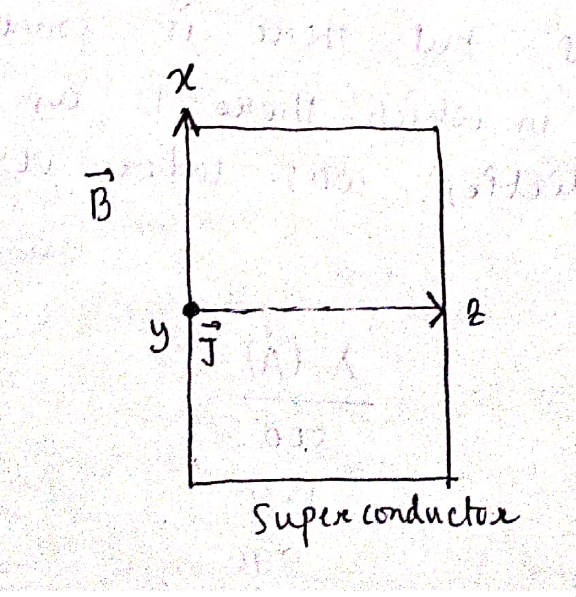
\includegraphics[width=0.5\textwidth]{figures/5.png}
    \end{center}
    \caption{Magnetic Field Decay from surface in superconductors}\label{fig:}
\end{figure}


\section{Magnetic Field Decay in Superconductors}

Equation (14) shows that the field decreases exponentially as one proceeds from the surface into the superconductor. Thus, the field vanishes inside the bulk of the medium, according to the Meissner effect.

This equation also tells us that the flux is not expelled entirely from the superconductor, as was once thought, but there is a small region near the surface in which there is an appreciable field. This prediction was later verified experimentally.

\section{Penetration Depth for Different Elements}

\begin{table}[h!]
\centering
\begin{tabular}{|c|c|}
\hline
\textbf{Element} & \(\lambda\) (\(\text{\AA}\)) \\ \hline
Al & 500 \\ \hline
Cd & 1300 \\ \hline
Pb & 390 \\ \hline
Sn & 510 \\ \hline
\end{tabular}
\caption{Penetration depth \(\lambda\) for different elements.}
\end{table}

\section{Temperature Dependence of the Penetration Depth}

Next, London's prediction is also verified with temperatures by the following empirical relation:
\[
\lambda = \lambda(0) \left[ 1 - \left( \frac{T^4}{T_c^4} \right) \right]^{-1/2}
\]
where
\[
\lambda(0) = \frac{mc^2}{\sqrt{4 \pi n_s e^2}}
\]
This equation shows the temperature dependence of the penetration depth \(\lambda\), and the graph illustrates the behavior of \(\lambda\) as the temperature approaches \(T_c\).

\begin{figure}
    \begin{center}
        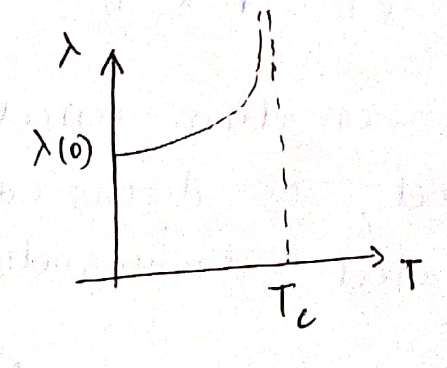
\includegraphics[width=0.45\textwidth]{figures/6.png}
    \end{center}
    \caption{London's Prediction and Empirical Formula}\label{fig:}
\end{figure}


\section{Third Conclusion: Surface Currents in Superconductors}

The current also decays exponentially as one moves into the superconductor:
\[
\vec{J}_y = \vec{J}_{y0} e^{-x/\lambda}
\]
This equation tells us that the current decays exponentially as one moves into the superconductor. Therefore, there exists a surface current. Finally, we can say that the Meissner effect is accompanied by a surface current, and it is this current that acts to shield the inner superconductor from the external magnetic field.

\section{Thermodynamics of Superconductors}

Let us consider a long, thin cylinder of superconducting material and place it in an external magnetic field of strength \(H\) that points along the cylinder axis. We know from the experiment of Meissner that for a critical field \(H_c\), the superconductivity is destroyed, and magnetic flux penetrates the sample, and the transition is completely reversible.

Therefore, at this critical field, the superconducting and normal state of the material must be in equilibrium. Thus, the free energy per unit volume of the material in the normal state is as follows:
\[
F = F_{\text{normal}} + \frac{B_c^2}{8 \pi \mu} \tag{15}
\]

Because the superconducting state expels the magnetic induction, its free energy is just \(F_{\text{superconducting}}\).

Above consideration suggests that \(F_{\text{normal}} > F_{\text{superconducting}}\) and the magnetic field energy is also true. But the way of thinking was wrong, since the thermodynamic tool is being used improperly. The reversible experiments are carried out by slowly varying external currents, not by controlling \(B\) directly.

\section{Thermodynamic Potential of Superconductors}

Therefore, the correct thermodynamic potential is:
\[
\tilde{F} \neq F
\]
\[
\tilde{F} = F - B \cdot \frac{\delta F}{\delta B}
\]
\[
\tilde{F} = F_{\text{normal}} - \frac{B_c^2}{8 \pi \mu} \tag{16}
\]

Therefore, the difference in free energy per unit volume at any given temperature between the superconducting and normal state must be exactly:
\[
\Delta F = F_{\text{normal}} - F_{\text{superconducting}} = \frac{B_c^2}{8 \pi \mu}
\]

For \(\mu = 1\) (for superconducting materials), we have:
\[
\Delta F = \frac{H_c^2}{8 \pi} \tag{17}
\]

Here, we know that the magnetic field \(H\) inside a long thin cylinder with the axis along the field is always spatially uniform and equal to the externally applied field. It is the magnetic induction \(B\) that is expelled from the superconducting sample, not the field \(H\).

By differentiating equation (3) with respect to temperature, we have the excess entropy of the normal metal relative to the superconductor:
\[
\Delta S = \frac{\partial}{\partial T} \Delta F = \frac{H_c}{4 \pi} \frac{\partial H_c}{\partial T} \tag{18}
\]

Meissner and Ochsenfeld determined that as the temperature \(T\) rises towards the critical temperature \(T_c\), where superconductivity vanishes with zero magnetic field, the critical field \(H_c\) also goes to zero. From equation (4), it can also be said that the latent heat of transformation is zero, and therefore the transition is second-order.

\section{Ginzburg-Landau Theory}

Landau and Ginzburg developed a theoretical framework to describe the superconducting state using a macroscopic wave function \(\psi\), analogous to the wave function \(\Psi\) in superfluid helium. Assuming that the supercurrent density \(n = |\psi|^2\) vanishes at the critical temperature \(T_c\), it is reasonable to expand the free energy in powers of \(|\psi|^2\). They proposed the Ginzburg-Landau free energy functional \(\mathcal{F}\) for a superconductor as:

\[
\mathcal{F} = \int d^3r \left[ \alpha |\psi|^2 + \frac{\beta}{2} |\psi|^4 + \frac{B^2}{8\pi} + \frac{1}{2m^*} \left| \left( \frac{\hbar}{i} \nabla + \frac{2e}{c} \mathbf{A}(r) \right) \psi(r) \right|^2 \right],
\]

where:

- \(\alpha\) and \(\beta\) are phenomenological parameters,
- \(B\) is the magnetic field,
- \(m^*\) is the effective mass of Cooper pairs,
- \(\mathbf{A}(r)\) is the electromagnetic vector potential,
- \(e\) is the elementary charge,
- \(c\) is the speed of light,
- \(\hbar\) is the reduced Planck constant.

The first two terms represent the condensation energy and come directly from Landau's general theory of second-order phase transitions. The third term accounts for the magnetic field energy, and the fourth term represents the kinetic energy associated with the superconducting current.

It is physically reasonable to assert that the macroscopic quantum wave function \(\psi(r)\) minimizes the free energy \(\mathcal{F}\). By treating \(\mathcal{F}\) as a functional of \(\psi(r)\) and employing the calculus of variations, we can derive differential equations governing the behavior of \(\psi(r)\) under equilibrium conditions.

The Helmholtz free energy of a superconductor includes three main contributions:

\[
F_s = F_n + \text{Condensation energy} + \text{Kinetic energy} + \text{Field energy},
\]

where \(F_n\) is the free energy in the normal state. This expression illustrates the general principle that the behavior of a superconductor results from a trade-off between the kinetic energy, field energy, and condensation energy.

Using the macroscopic quantum model, we can express the free energy as:

\[
F_s = F_n + \int d^3r \left[ f_0 + \frac{1}{2m^*} \left| \left( -i \hbar \nabla - \frac{e^*}{c} \mathbf{A} \right) \psi \right|^2 \right] + \int d^3r \frac{B^2}{8\pi},
\]

where \(f_0\) represents the condensation free energy density, and \(e^* = 2e\) is the effective charge of a Cooper pair.

To gain insight into the kinetic energy density term, consider the wave function in polar form:

\[
\psi(r) = |\psi(r)| e^{i \phi(r)}.
\]

Substituting this into the kinetic energy term yields:

\[
\text{Kinetic Energy} = \frac{1}{2m^*} \left[ \hbar^2 (\nabla |\psi|)^2 + |\psi|^2 \left( \hbar \nabla \phi - \frac{e^*}{c} \mathbf{A} \right)^2 \right].
\]

This expression shows that the kinetic energy density includes contributions from spatial variations in both the amplitude \(|\psi|\) and the phase \(\phi\) of the wave function. The gradient term \(\nabla |\psi|\) introduces new physics not captured by the London theory, highlighting the importance of spatial variations in the superconducting order parameter.

Recognizing that the condensation energy must depend on the density of superconducting pairs, we generalize the free energy to:

\[
F_{GL}\{\psi(r), \psi^*(r), \mathbf{A}\} = F_n + \int d^3r \left\{ f_0(|\psi|^2) + \frac{1}{2m^*} \left| \left( -i \hbar \nabla - \frac{e^*}{c} \mathbf{A} \right) \psi \right|^2 + \frac{(\nabla \times \mathbf{A})^2}{8\pi} \right\},
\]

where \(f_0(|\psi|^2)\) now explicitly depends on \(|\psi|^2\).

Since the exact functional form of \(f_0(|\psi|^2)\) is not known \emph{a priori}, Ginzburg and Landau expanded it as a Taylor series in powers of \(|\psi|^2\):

\[
f_0(|\psi|^2) = \alpha |\psi|^2 + \frac{\beta}{2} |\psi|^4,
\]

\begin{figure}
    \begin{center}
        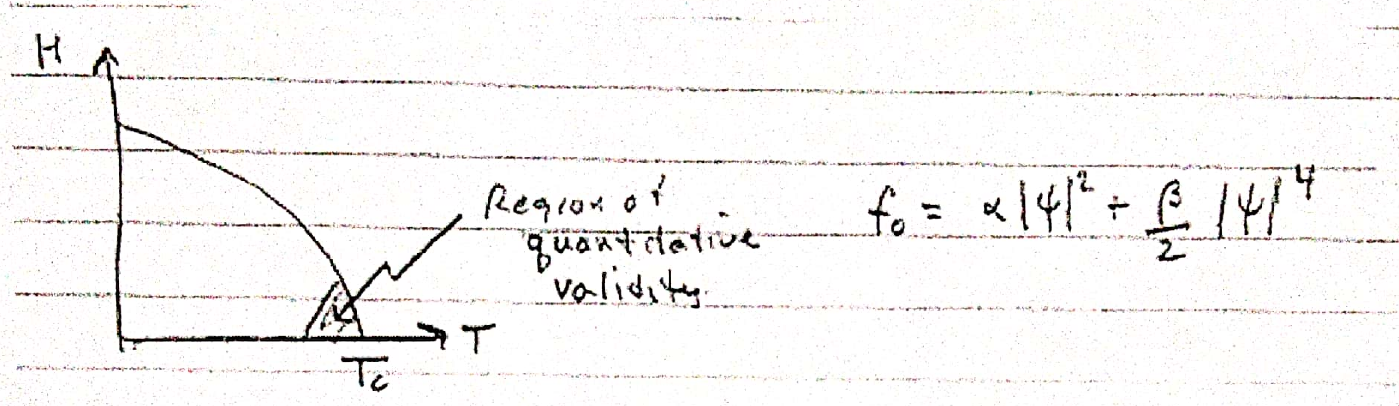
\includegraphics[width=0.95\textwidth]{figures/8.png}
    \end{center}
    \caption{Superconductivity in terms of empirical formula}\label{fig:}
\end{figure}


where \(\alpha\) and \(\beta\) are phenomenological coefficients to be determined experimentally. In the case of classic BCS superconductors, these parameters can also be calculated from the microscopic theory.

This expansion is justified near the critical temperature \(T_c\), where \(|\psi|^2\) is small and varies slowly in space, making higher-order terms negligible. Although the theory is most accurate near \(T_c\), it remains qualitatively useful over a broader temperature range and provides valuable insights into the behavior of superconductors.

By incorporating this expression for \(f_0\), the Ginzburg-Landau free energy functional becomes:

\[
\mathcal{F}_{GL} = F_n + \int d^3r \left[ \alpha |\psi|^2 + \frac{\beta}{2} |\psi|^4 + \frac{1}{2m^*} \left| \left( -i \hbar \nabla - \frac{e^*}{c} \mathbf{A} \right) \psi \right|^2 + \frac{B^2}{8\pi} \right].
\]

This formulation captures the essential physics of superconductivity by balancing the condensation energy with kinetic and magnetic energies. It highlights that the behavior of a superconductor results from a trade-off between these energies, governed by the spatial variation and magnitude of the superconducting order parameter \(\psi(r)\). 

\begin{theorem}
\textbf{Explanation of the Terms:}

1. \(\alpha |\psi|^2\):
   This term represents the free energy contribution from the magnitude of the order parameter \(\psi\). The coefficient \(\alpha\) typically changes sign at the critical temperature \(T_c\). For \(T > T_c\), \(\alpha > 0\) (normal state), and for \(T < T_c\), \(\alpha < 0\) (superconducting state). The order parameter \(\psi\) describes the density of superconducting pairs.

2. \(\frac{\beta}{2} |\psi|^4\): 
   This is a nonlinear term, which prevents the magnitude of \(\psi\) from growing indefinitely. The coefficient \(\beta\) is positive, ensuring that the free energy has a minimum for a non-zero value of \(\psi\) when \(\alpha < 0\), corresponding to the superconducting state.

3. \(\frac{B^2}{8\pi}\):
   This term represents the energy stored in the magnetic field \(\mathbf{B}\). In the absence of external fields, the magnetic field is expelled from the superconductor (Meissner effect), but in type-II superconductors, magnetic fields can penetrate in the form of vortices.

4. \(\frac{1}{2m^*} \left| \left( \frac{\hbar}{i} \nabla + \frac{2e}{c} \mathbf{A}(r) \right) \psi(r) \right|^2\): 
   This term describes the kinetic energy of the superconducting electrons (Cooper pairs). The operator \(\frac{\hbar}{i} \nabla\) is the momentum operator, and the term \(\frac{2e}{c} \mathbf{A}(r)\) accounts for the coupling of the superconducting wavefunction \(\psi\) to the electromagnetic vector potential \(\mathbf{A}(r)\).

   - \(\frac{\hbar}{i} \nabla\): This is the canonical momentum operator, acting on the wavefunction \(\psi\).
   - \(\frac{2e}{c} \mathbf{A}(r)\): This term arises due to the interaction between the superconducting current and the magnetic field. The factor of \(2e\) corresponds to the charge of a Cooper pair, which consists of two electrons (each with charge \(-e\), so the total charge is \(2e\)).

   \textbf{ Why is there \(2e/c\) in the potential?}

The factor \(2e/c\) appears because the order parameter \(\psi\) describes Cooper pairs, not individual electrons. Each Cooper pair has a total charge of \(2e\), and the magnetic vector potential \(\mathbf{A}\) couples to this total charge in the same way the electromagnetic potential couples to a charged particle in the presence of a magnetic field. The factor \(c\) appears because the electromagnetic potential is in cgs units, where the speed of light is involved in relating the vector potential to the magnetic field.

In summary, the term \(\frac{2e}{c} \mathbf{A}(r)\) represents the interaction between the Cooper pairs (with charge \(2e\)) and the electromagnetic vector potential \(\mathbf{A}\), which mediates the influence of the magnetic field on the supercurrent in the superconductor.
    
\end{theorem}


\section{Ginzburg-Landau Theory for Superconductors}

\begin{itemize}
    \item Canonical momentum has to be replaced by the kinetic momentum:
    \[
    \frac{\hbar}{i} \nabla \rightarrow \frac{\hbar}{i} \nabla + \frac{2e}{c} \mathbf{A}
    \]
    where $\mathbf{A}$ is the vector potential.

    \item The energy density of the magnetic field, $B^2 / 8\pi$, has to be included.

    \item The Ginzburg-Landau free energy functional $F_{GL} \{ \psi(r), \psi^*(r), \mathbf{A} \}$ is given by:
    \begin{equation}
    F_{GL} \{ \psi(r), \psi^*(r), \mathbf{A} \} = F_n + \int d^3r \left[ \alpha |\psi|^2 + \frac{\beta}{2} |\psi|^4 + \frac{B^2}{8\pi} + \frac{1}{2m^*} \left( \frac{\hbar}{i} \nabla + \frac{2e}{c} \mathbf{A} \right) |\psi|^2 \right]
    \end{equation}
\end{itemize}

Minimizing the free energy with respect to $\psi^*$:

\begin{equation}
    \frac{1}{2m^*} \left( \frac{\hbar}{i} \nabla + \frac{2e}{c} \mathbf{A} \right)^2 \psi + \alpha \psi + \beta |\psi|^2 \psi = 0
\end{equation}

To minimize $F_{GL}$ with respect to $\mathbf{A}$, we write $\mathbf{A}(r) = \mathbf{A}_0(r) + \mathbf{a}(r)$ and substitute this into the terms containing $\mathbf{A}$:

\begin{equation}
    F_{GL} \{ \psi(r), \psi^*(r), \mathbf{A}_0 + \mathbf{a}(r) \} = F_n \{ \psi, \psi^*, \mathbf{A}_0 \} + [ \int d^3r \left[ \frac{1}{2m^*} \left( \frac{\hbar}{i} \nabla + \frac{2e}{c} \mathbf{A}_0 \right)\psi \right]^* \cdot \left( \frac{2e}{c} \mathbf{a} \psi \right)
\end{equation}

\begin{equation}
+ \frac{1}{2m^*} \left( \frac{2e}{c} \mathbf{a} \psi \right)^* \cdot \left( \frac{\hbar}{i} \nabla + \frac{2e}{c} \mathbf{A}_0 \right) \psi + \frac{1}{4\pi} (\nabla \times \mathbf{A}_0) \cdot (\nabla \times \mathbf{a}) ]
\end{equation}

\[
(\nabla \times \mathbf{A}_0) \cdot (\nabla \times \mathbf{a}) = \mathbf{a} \cdot (\nabla \times \nabla \times \mathbf{A}_0) - \nabla \cdot \left[ (\nabla \times \mathbf{A}_0) \times \mathbf{a} \right] = 0
\]

The Ginzburg-Landau free energy functional is then expressed as:

\begin{equation}
    F_{GL} \{ \psi, \psi^*, \mathbf{A} \} = F \{ \psi, \psi^*, \mathbf{A}_0 \} + \int d^3r \left[ \frac{e}{m^* c} \left( \frac{\hbar}{i} \nabla \psi \right)^* \psi +  \psi^*    \frac{\hbar}{i} \nabla \psi \right] \cdot \mathbf{a}
\end{equation}

\begin{equation}
    + \frac{4 e^2}{m^* c^2} |\psi|^2 \mathbf{A}_0 \cdot \mathbf{a} + \frac{1}{4\pi} (\nabla \times \mathbf{B}_0) \cdot \mathbf{a} + O(a^2)
\end{equation}

Applying the variational technique, we have from equation (3):

\begin{equation}
    \frac{e \hbar}{m^* c i} \left( -\psi \nabla \psi^* + \psi^* \nabla \psi \right) + \frac{4 e^2}{m^* c^2} |\psi|^2 \mathbf{A} + \frac{1}{4\pi} \nabla \times \mathbf{B} = 0
\end{equation}

or,

\begin{equation}
    - \frac{i e \hbar}{m^* c} \left( \psi^* \nabla \psi - \psi \nabla \psi^* \right) + \frac{4 e^2}{m^* c^2} |\psi|^2 \mathbf{A} + \frac{1}{4\pi} \nabla \times \mathbf{B} = 0 \tag{19}
\end{equation}

We know:

\[
    \nabla \times \mathbf{B} = \frac{4\pi}{c} \mathbf{J}
\]

Applying this to equation (4) gives:

\begin{equation}
    - \frac{i e \hbar}{m^*} \left( \psi^* \nabla \psi - \psi \nabla \psi^* \right) + \frac{4 e^2}{m^* c} |\psi|^2 \mathbf{A} + \mathbf{J} = 0
\end{equation}

or,

\begin{equation}
    \mathbf{J} = \frac{i e \hbar}{m^* c} \left( \psi^* \nabla \psi - \psi \nabla \psi^* \right) - \frac{4 e^2}{m^* c} |\psi|^2 \mathbf{A} \tag{20}
\end{equation}

\begin{theorem}
The Ginzburg-Landau equations describe the behavior of superconductors near the transition temperature. These equations are derived from the Ginzburg-Landau free energy functional by minimizing with respect to the order parameter $\psi$ and the vector potential $\mathbf{A}$.

\subsection*{First Ginzburg-Landau Equation}
Minimizing the free energy with respect to $\psi^*$ gives the first Ginzburg-Landau equation:
\begin{equation}
    \frac{1}{2m^*} \left( \frac{\hbar}{i} \nabla + \frac{2e}{c} \mathbf{A} \right)^2 \psi + \alpha \psi + \beta |\psi|^2 \psi = 0
\end{equation}
This equation governs the spatial variation of the superconducting order parameter $\psi$.

\subsection*{Second Ginzburg-Landau Equation}
Minimizing the free energy with respect to $\mathbf{A}$ leads to the second Ginzburg-Landau equation, which relates the supercurrent density $\mathbf{J}$ to $\psi$ and $\mathbf{A}$:
\begin{equation}
    \mathbf{J} = \frac{i e \hbar}{m^* c} \left( \psi^* \nabla \psi - \psi \nabla \psi^* \right) - \frac{4 e^2}{m^* c} |\psi|^2 \mathbf{A}
\end{equation}

The Ginzburg-Landau equations describe the macroscopic properties of superconductors, providing insight into phenomena like the Meissner effect and vortex formation in type-II superconductors.

\end{theorem}

\section{Boundary Condition}

When deriving from the variational process, we also get an expression for the boundary conditions at any superconductor/vacuum interface:
\begin{equation}
    \left( \frac{\hbar}{i} \nabla + \frac{2e}{c} \mathbf{A} \right) \cdot \hat{n} = 0 \tag{21}
\end{equation}

Here, $\hat{n}$ is the normal to the boundary. Equation (6) ensures that $\mathbf{J}_s \cdot \hat{n} = 0$ at the surface, meaning there is no current flow out of the boundary (no current leakage across the boundary).

\section{Free Energy in the London Limit}

To make the connection to the London theory explicit, if $n_s^*$ is a constant, 
\[
F_s = F_n = \int d^3r \left\{ f_0 + n_s^* \frac{1}{2} m^* v_s^2 + \frac{1}{8\pi} h^2 \right\} \tag{25}
\]
which is intuitively appealing.

Also, using $v_s = J_s / n_s^* e^*$ and the definition of $\lambda$, the kinetic energy term can be written:
\[
n_s^* \frac{1}{2} m^* v_s^2 = \frac{1}{2} \frac{4\pi \lambda^2}{c^2} J_s^2 = \frac{\lambda^2}{8\pi} (\nabla \times h)^2 \tag{26}
\]
and the free energy can be written in the particularly compact and useful form:
\[
F_s = F_n = \int d^3r \left\{ -\frac{H_c^2}{8\pi} + \frac{1}{8\pi} \left[ \lambda^2 (\nabla \times h)^2 + h^2 \right] \right\} \tag{27}
\]

Finally, note that the kinetic energy density can also be written:
\[
n_s^* \frac{1}{2} m^* v_s^2 = \frac{1}{2} \mathcal{L}_K J_s^2 \tag{28}
\]
which emphasizes that the kinetic energy is an inductive stored energy.

\section{Equilibrium value of $|\psi|$ and determination of the material parameters}

As noted above, the parameters of the Ginzburg-Landau theory can be determined from experiment. Neglecting fields and currents, we know that the minimum of $f_0(|\psi|^2)$ must give the equilibrium condensation energy and the equilibrium pair density. The former can be measured directly, and the latter can be determined from a measurement of the penetration depth.

\begin{figure}
    \begin{center}
        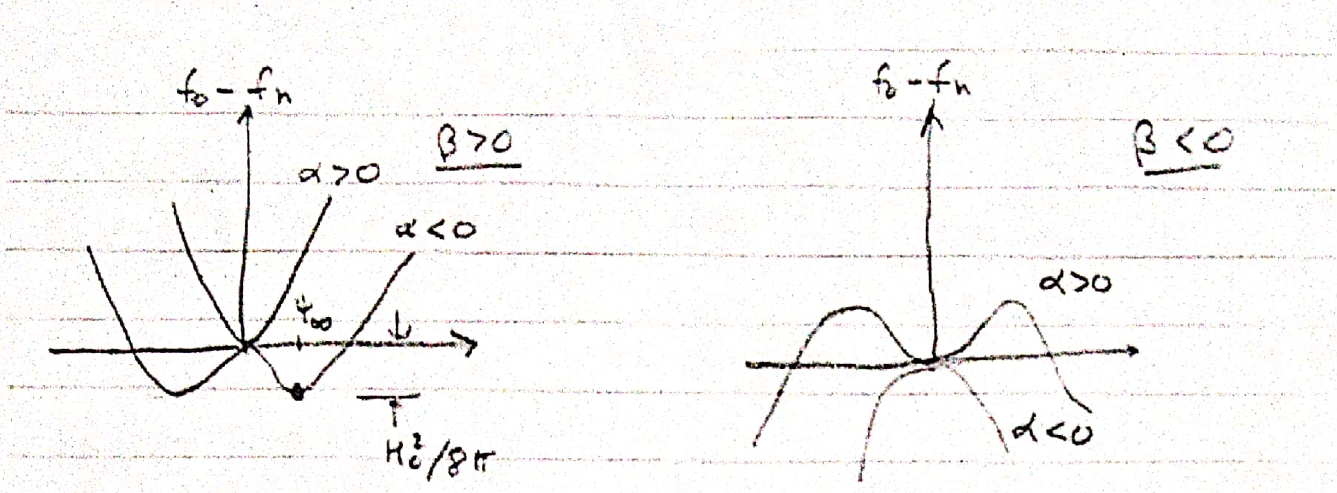
\includegraphics[width=0.95\textwidth]{figures/9.png}
    \end{center}
    \caption{Material parameters in Ginzburg-Landau Theory}\label{fig:}
\end{figure}

Consider the structure of $f_0$ as a function of $\psi$, depending on the signs of $\alpha$ and $\beta$, as illustrated in Fig. 4.2. Clearly, only $\beta > 0$ is physical. Moreover, when $\alpha > 0$, clearly the minimum (i.e., the equilibrium state) corresponds to the normal state, $|\psi_{\text{eq}}| = 0$. However, when $\alpha < 0$, the superconducting state is stable, $|\psi_{\text{eq}}| > 0$. We conclude, therefore, that $\alpha(T)$ must change sign at $T = T_c$. Following Ginzburg and Landau, we take

\[
\alpha(T) = \alpha_0 \left( \frac{T - T_c}{T_c} \right) = \alpha_0 (t - 1) \tag{31}
\]
and $\beta$ is independent of temperature. As we shall see, these choices are consistent with experiment.


Note that in the figure above, when viewed as functions of $\psi$ as opposed to $|\psi|$, the curves are sections through the full free energy density space. In this case, the single x-axis becomes a plane in $\text{Re} \, \psi$ and $\text{Im} \, \psi$ space, and the full free energy curve is just a rotation of the curve shown around the z-axis. The point is that the overall phase of the wave function is arbitrary.

It is trivial to determine the equilibrium value of $|\psi|$ in the superconducting state ($\alpha < 0$), which is traditionally designated as $\psi_\infty$ (see Fig. 4.2). Taking

\[
\frac{\partial f}{\partial |\psi|} = 2 \alpha |\psi| + 2 \beta |\psi|^3 = 0 \tag{32}
\]
to find the minimum, yields
\[
\psi_\infty^2 = -\frac{\alpha}{\beta} = \frac{|\alpha|}{\beta} \tag{33}
\]

In addition, the equilibrium condensation energy density is given by:

\[
(f_s - f_n) \bigg|_{|\psi| = \psi_\infty} = - \frac{\alpha^2}{2\beta} \tag{34}
\]

These expressions can be easily related to experiment in order to determine $\alpha$ and $\beta$. Since
\[
\lambda^2 = \frac{m^* c^2}{4\pi e^2 n_s^*} \tag{35}
\]
it follows that
\[
\psi_\infty^2 = \frac{|\alpha|}{\beta} = \frac{m^* c^2}{4\pi e^2 \lambda^2} \tag{36}
\]
and directly, we have
\[
(f_s - f_n) \bigg|_{|\psi| = \psi_\infty} = - \frac{\alpha^2}{2\beta} = - \frac{H_c^2}{8\pi} \tag{37}
\]

Taken together, these two results yield
\[
|\alpha| = \frac{e^2 H_c^2 \lambda^2}{m^* c^2} \propto (1 - t) \tag{38}
\]

Note that the temperature dependences of $\alpha$ and $\beta$ determined from experiment are consistent with those assumed initially, confirming those assumptions.

\section{Physical content of the Ginzburg-Landau equations}

Pondering these equations, we see that the second GL equation (for $\mathbf{J}_s$) is exactly that obtained in the macroscopic quantum model, as it must be, only here we see that it is consistent with minimization of the free energy. It is the first GL equation that contains the new physics. Specifically, it governs the spatial variations of $\psi$. Associated with these spatial variations is a new length scale — the so-called GL coherence length $\xi(T)$ — that governs the distance over which $\psi$ naturally varies 

\section{Coherence length, $\xi$}

From equation (2), we know from earlier that the value of $\beta$ is always positive and $\alpha > 0$ for the normal state and $\alpha < 0$ for the superconducting state. Let us consider a case in which externally imposed magnetic fields vanish, and hence the solutions of equation (2) are:

\[
|\psi|^2 = 
\begin{cases}
    \psi_0^2 = -\frac{\alpha}{\beta}, \\
    0
\end{cases} \tag{39}
\]

As we said earlier, taking
\[
\frac{\partial F}{\partial |\psi|} = 2 \alpha |\psi| + 2 \beta |\psi|^3 = 0
\]
we obtain
\[
\psi_0^2 = - \frac{\alpha}{\beta} = \frac{|\alpha|}{\beta}
\]
since $\alpha < 0$ for the superconducting state.

In addition, the equilibrium condensation energy density is given by
\[
(f_s - f_n)\bigg|_{|\psi| = \psi_0} = - \frac{\alpha^2}{2\beta} = \Delta f \tag{40}
\]

Comparing with equation $\Delta f = \frac{H_c^2}{8\pi}$, we can write
\[
H_c^2 = \frac{4 \pi \alpha^2}{\beta} \tag{41}
\]

\section{Case: When $\mathbf{A}$ is zero}

When $\mathbf{A}$ is zero, the Ginzburg-Landau (GL) equation (2) can be written as:
\[
-\frac{\hbar^2}{2m^*} \nabla^2 \psi + \alpha \psi + \beta |\psi|^2 \psi = 0 \tag{12}
\]

This equation is very similar to the time-independent Schrödinger equation, but interestingly, it contains a non-linear term. Now, we apply it to find the variation of $\psi(r)$ in the superconductor, close to the surface. When superconductivity is present, it makes sense to scale $\psi$ by this uniform value $\psi_0 = \sqrt{-\alpha/\beta}$. Let us consider a one-dimensional lattice and assume that the solution depends only on $x$. Then equation (12) becomes:
\[
-\frac{\hbar^2}{2m^*} \frac{d^2 \psi(x)}{dx^2} + \alpha \psi(x) + \beta |\psi(x)|^2 \psi(x) = 0 \tag{13}
\]

Since all coefficients are real, the solution can be chosen real. For $x \to \infty$, we should obtain the uniform solution:
\[
\lim_{x \to \infty} \psi(x) = \sqrt{-\frac{\alpha}{\beta}}
\]
Writing
\[
\psi(x) = \sqrt{-\frac{\alpha}{\beta}} f(x) \tag{14}
\]
Applying this above, equation (13) becomes:
\[
-\frac{\hbar^2}{2m^* \alpha} f''(x) + f(x) - f(x)^3 = 0 \tag{15}
\]

Equation (15) contains a characteristic length, $\xi$, with
\[
\xi^2 = -\frac{\hbar^2}{2m^*\alpha} = \frac{\hbar^2}{2m^* |\alpha|} \sim \frac{\hbar^2}{2m^* \alpha_0' (T_C - T)} > 0
\]
which is called the Ginzburg-Landau coherence length. The Ginzburg-Landau coherence length, $\xi$, has a strong temperature dependence and actually diverges as $T \to T_C$.

Multiplying equation (15) by $f(x)$ and integrating, we obtain the integral:
\[
-\xi^2 \left(f'(x)\right)^2 - \left(f(x)\right)^2 + \frac{1}{2} \left(f(x)\right)^4 = \text{constant} \tag{16}
\]
For a value of $f(x) = 1$, the constant should be $-\frac{1}{2}$ on the RHS. In this case, from (16), we can obtain:
\[
f'(x) = \frac{1}{\sqrt{2}\xi} \left(1 - f(x)^2\right)
\]
which has the solution:
\[
f(x) = \tanh\left(\frac{x}{\sqrt{2}\xi}\right) \tag{17}
\]
Thus, we have:
\[
\psi(x) = \sqrt{\frac{-\alpha}{\beta}} \tanh\left(\frac{x}{\sqrt{2}\xi}\right)
\]

\begin{figure}
    \begin{center}
        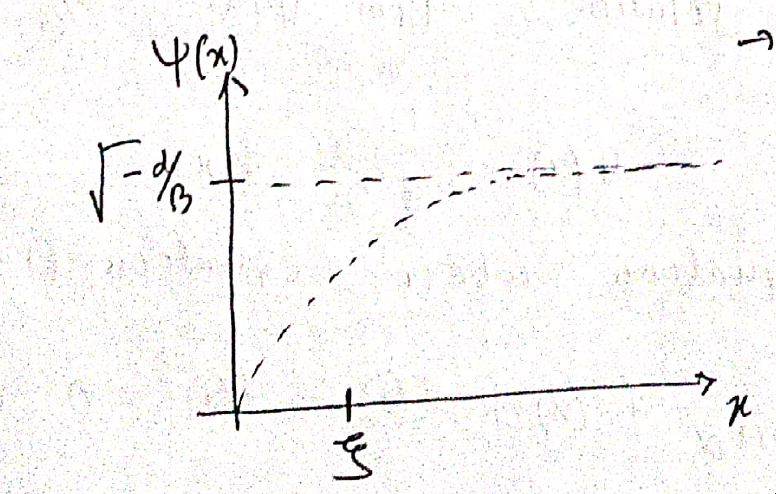
\includegraphics[width=0.65\textwidth]{figures/7.png}
    \end{center}
    \caption{Solution when there is no magnetization}\label{fig:}
\end{figure}


This solution describes a transition between two spatially uniform superconducting regions where the phase of the wave function changes sign across the interface. The coherence length $\xi$ sets the spatial scale for this transition.

\section{Penetration Depth}
It arises when one considers a superconductor occupying the region, say $x < 0$, in an exceedingly weak field. When the field is zero, one has the solution $\psi = \psi_0$ for $x < 0$. In the presence of a very weak field, $\psi$ will change to linear order in the field, but it is non-zero without a field. To the leading order, one can continue with $\psi = \psi_0$. Keeping only the leading terms, equation (5) gives:
\[
\mathbf{J} = \frac{c}{4\pi} \nabla \times \mathbf{B} = -\frac{4e^2}{m^* c} \psi_0^2 \mathbf{A} \tag{8}
\]
Taking the curl of the above equation:
\[
\nabla \times \left( \nabla \times \mathbf{B} \right) = -\frac{4\pi}{c} \frac{4e^2}{m^* c} \psi_0^2 \mathbf{B} = \frac{1}{\lambda_L^2} \mathbf{B} \tag{19}
\]
where
\[
\lambda_L^2 = \frac{m^* c^2 \beta}{4 \pi |\alpha| (2e)^2} \tag{20}
\]
is the London penetration depth.

\section{Ratio of Penetration Depth and Coherence Length}
The ratio of the penetration depth and the coherence length can be written as:
\[
\kappa = \frac{\lambda_L}{\xi} = \frac{m^* c}{e\hbar} \sqrt{\frac{\beta}{8\pi}} \tag{21}
\]

Let us define:
\[
\tilde{\mathbf{A}} = \frac{4e \mathbf{A}}{c \sqrt{2m^* \alpha}} \tag{22}
\]
Equation (2) gives:
\[
\psi = |\psi|^2 - \left( -i \nabla + \tilde{\mathbf{A}}/2 \right)^2 \psi = 0 \tag{23}
\]
While equation (5) becomes:
\[
\frac{\lambda_L^2}{\xi^2} \left( \nabla \times \nabla \times \tilde{\mathbf{A}} \right) - \frac{1}{i} \left( \psi^2 \nabla \psi - \psi \nabla \psi^* \right) - \tilde{\mathbf{A}} \psi^2 = 0 \tag{24}
\]


\end{document}
 
